Introduce a curve into \hyperref[CSX]{\matv{CSX}} with matlab function \texttt{AddCurve} and assign a property to it. 

\begin{FontNameFunct}{AddCurve()}
\end{FontNameFunct}


\begin{FontDescr}{Purpose:}
Add 1D curve to \hyperref[CSX]{\matv{CSX}} by defining its coordinate arrays.
\end{FontDescr}

\begin{FontDescr}{Syntax:}
\begin{lstlisting} 
 CSX = AddCurve(CSX, propName, prio, points, varargin)
\end{lstlisting}
\end{FontDescr}

\begin{FontDescr}{Description:}

\begin{FontPara}{propName}
Refer to \hyperref[prim_Name]{propName} in \texttt{AddBox}. 
\end{FontPara}

\begin{FontPara}{points}
\phantomsection \label{points_curve}
Curve coordinates array. Array column refers to point number while array row refers to its x,y,z- position:
\begin{myindentpar}     
points(1,point$\_$number): position-x of point.\\
points(2,point$\_$number): position-y of point.\\
points(3,point$\_$number): position-z of point.
\end{myindentpar}

\end{FontPara}
\end{FontDescr}

\begin{FontDescr}{Optional Arguments:}
The standard trasformation (rotation,translation,scaling) mentioned in  \hyperref[prim_transform]{\matv{'Transform'}} of \texttt{AddBox}.   
\end{FontDescr}


\begin{FontDescr}{Examples:}

\begin{lstlisting} 
%first point
     points(1,1) = 0;points(2,1) = 5;points(3,1) = 10; 
%second point
     points(1,2) = 0;points(2,2) = 10;points(3,2) = 10; 
     CSX = AddMetal(CSX,'metal'); 
     CSX = AddCurve(CSX,'metal',10, points);
\end{lstlisting}
This example creates a thin metallic wire from y=5 to y=10(5 drawing unit long).

\begin{lstlisting} 
    points(1,1) =  0;points(2,1) = 0;points(3,1) = 0;
    points(1,2) =  5;points(2,2) = 0;points(3,2) = 5;
    points(1,3) = 10;points(2,3) = 0;points(3,3) = 0.5;
    points(1,4) = 15;points(2,4) = 0;points(3,4) = 5;
    points(1,5) = 20;points(2,5) = 0;points(3,5) = 0;
    points(1,6) = 15;points(2,6) = 0;points(3,6) = -5;
    points(1,7) = 10;points(2,7) = 0;points(3,7) = -0.1;
    points(1,8) =  5;points(2,8) = 0;points(3,8) = -5;
    points(1,9) =  0;points(2,9) = 0;points(3,9) = 0;
    CSX = AddMetal(CSX,'metal'); 
    CSX = AddCurve(CSX,'metal',10, points);
\end{lstlisting}
This example creates a Biquad antenna from thin wire on y=0, with length of each side=$\sqrt{50}$.
\end{FontDescr}

\begin{figure}[hbt]
\centering
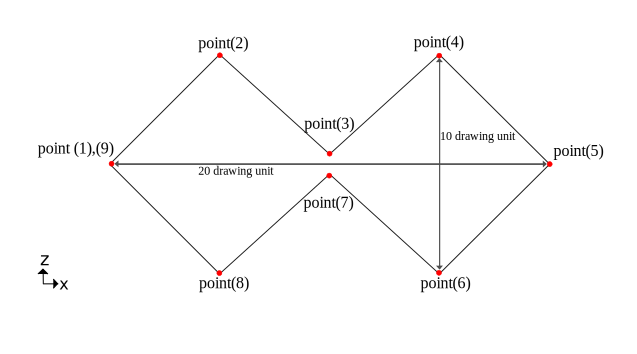
\includegraphics[width=0.8\textwidth]{svg/biquad_prim_curve.pdf}
\caption{Biquad antenna with side length $\sqrt{50}$ in xz-plane.}
\label{fig:primCurve}
\end{figure}